\documentclass[pdftex]{beamer}
%\input{vc}
% 1.77778 is the ratio of 16 to 9
\setlength{\paperheight}{3.5in}
\setlength{\paperwidth}{1.77778\paperheight}
% 1.33333 is the ratio of 4 to 3
%\setlength{\paperheight}{4.0in}
%\setlength{\paperwidth}{1.33333\paperheight}
\setlength{\textwidth}{0.85\paperwidth}
% import the next thing *after* the papersize
\usepackage{amssymb,amsmath,mathrsfs}
\usecolortheme{default}

% this one is debatable
\renewcommand{\emph}[1]{\textbf{#1}}

%%% color commands
\newcommand{\whiteonblack}{%
  \colorlet{fg}{white}
  \colorlet{bg}{black}
  \setbeamercolor{normal_text}{fg=white,bg=black}
  \setbeamercolor{background canvas}{fg=white,bg=black}
  \setbeamercolor{alerted_text}{fg=yellow}
  \setbeamercolor{example_text}{fg=white}
  \setbeamercolor{structure}{fg=white}
  \setbeamercolor{palette_quaternary}{fg=white}
}
\newcommand{\blackonwhite}{%
  \colorlet{fg}{black}
  \colorlet{bg}{white}
  \setbeamercolor{normal_text}{fg=black,bg=white}
  \setbeamercolor{background canvas}{fg=black,bg=white}
  \setbeamercolor{alerted_text}{fg=blue}
  \setbeamercolor{example_text}{fg=black}
  \setbeamercolor{structure}{fg=black}
  \setbeamercolor{palette_quaternary}{fg=black}
}
\xdefinecolor{pink}{rgb}{1.0,0.9,0.9}

%%% size and shape commands
\newlength{\figurewidth}
\setlength{\figurewidth}{\textwidth}
\newlength{\figureheight}
\setlength{\figureheight}{0.9\textheight}

%%% text commands
\newcommand{\project}[1]{\textsl{#1}}
  \newcommand{\tc}{\project{The~Cannon}}
  \newcommand{\an}{\project{Astrometry.net}}
  \newcommand{\euclid}{\project{Euclid}}
  \newcommand{\flickr}{\project{flickr}}
  \newcommand{\gaia}{\project{Gaia}}
  \newcommand{\galex}{\project{GALEX}}
  \newcommand{\kepler}{\project{Kepler}}
  \newcommand{\GALEX}{\galex}
  \newcommand{\hst}{\project{HST}}
  \newcommand{\hipparcos}{\project{Hipparcos}}
  \newcommand{\lsst}{\project{LSST}}
  \newcommand{\sdss}{\project{SDSS}}
  \newcommand{\sdssiii}{\project{SDSS-III}}
  \newcommand{\sdssiv}{\project{SDSS-IV}}
  \newcommand{\boss}{\project{BOSS}}
  \newcommand{\apogee}{\project{APOGEE}}
  \newcommand{\osss}{\project{OSSS}}
  \newcommand{\ska}{\project{SKA}}
  \newcommand{\vo}{\project{VO}}
  \newcommand{\rttd}{\project{Right Thing To Do}$^{\mbox{\scriptsize\sffamily{TM}}}$}
\newcommand{\foreign}[1]{\textit{#1}}
\newcommand{\latin}[1]{\foreign{#1}}
  \newcommand{\cf}{\latin{cf.}}
  \newcommand{\eg}{\latin{e.g.}}
  \newcommand{\etal}{\latin{et~al.}}
  \newcommand{\etc}{\latin{etc.}}
  \newcommand{\ie}{\latin{i.e.}}
  \newcommand{\vs}{\latin{vs.}}

%%% math-mode commands
\newcommand{\unit}[1]{\mathrm{#1}}
  \newcommand{\rad}{\unit{rad}}
  \newcommand{\s}{\unit{s}}
  \newcommand{\yr}{\unit{yr}}
  \newcommand{\km}{\unit{km}}
  \newcommand{\kmps}{\km\,\s^{-1}}
\newcommand{\mmatrix}[1]{\boldsymbol{#1}}
\newcommand{\tv}[1]{\boldsymbol{#1}}
\newcommand{\dd}{\mathrm{d}}
\newcommand{\given}{\,|\,}
\newcommand{\transpose}[1]{{#1}^{\mathsf{\!T}}}
\DeclareMathOperator*{\diag}{diag}
 % hogg standard colors

\title{The theory and practice of self-calibration}
\author[David W. Hogg (NYU)]{David W. Hogg \\
  \textsl{\small Center for Cosmology and Particle Physics,
                 New York University} \\
  \textsl{\small Center for Data Science,
                 New York University} \\
  \textsl{\small Max-Planck-Insitut f\"ur Astronomie, Heidelberg}}
\date{2015 May 20}

\newcommand{\conclusions}{%
\begin{frame}
  \frametitle{summary}
  \begin{itemize}
  \item \sdss\ switched from a standards-based calibration to self-calibration.
    \begin{itemize}
    \item \emph{no use of standard stars} whatsoever (except\ldots)
    \item extremely successful (exceeds spec)
    \item required certain kinds of non-trivial observational redundancy
    \end{itemize}
  \item New surveys plan single-pass wide-field imaging surveys.
    \begin{itemize}
    \item \euclid, \wfirst
    \item imaging with a repeated dither pattern on a grid is a \emph{bad, bad idea}
    \item patterns far better for calibration can be equally efficient
    \end{itemize}
  \item Ideas from causal inference bring new, far crazier ideas to self-calibration.
    \begin{itemize}
    \item surveys that \emph{never repeat} and have \emph{no redundancy}
    \item \kepler\ and \kt\ lightcurves
    \item \wfc\ flat-field
    \end{itemize}
  \end{itemize}
\end{frame}}

\begin{document}

\conclusions

\begin{frame}
  \titlepage
\end{frame}

\begin{frame}
  \frametitle{Potted \sdss\ calibration history}
  \begin{itemize}
  \item original plan was to calibrate (with the \project{PT}) a network of standard stars
  \item flat-field obtained by ``sky flat''
    \begin{itemize}
    \item \emph{this is generally a terrible idea!}
    \end{itemize}
  \item realized that there was a huge amount of calibration information in the science data
    \begin{itemize}
    \item consistency requirements are incredibly constraining
    \item \emph{we ordered cross-scans}
    \end{itemize}
  \item Roweis showed us how to tractably fit a huge model to all the science data
  \item \project{PT} became a (very valuable) photometricity monitor
    \begin{itemize}
    \item my most highly cited first-author paper!
    \item there is no use of the original calibration program in post-DR8 \sdss\ data
    \end{itemize}
  \end{itemize}
\end{frame}

\begin{frame}
  \frametitle{\sdss\ self-calibration {\footnotesize (Padmanabhan \etal, arXiv:XXX)}}
  ~\hfill%
  \includegraphics<1>[width=0.8\figurewidth]{./0703454v2/geom.pdf}
  \includegraphics<2>[width=0.95\figurewidth]{./0703454v2/sky_coverage.pdf}
\end{frame}

\begin{frame}
  \frametitle{\sdss\ self-calibration {\footnotesize (Padmanabhan \etal, arXiv:XXX)}}
  \begin{eqnarray}
  \chi^2 &=& \sum_i \chi_i^2 \\
  \chi_i^2 &=& \sum_{j\in O_i} \frac{[2.5\,\log C_{ij} + m_i - a_j - k(t_{ij})\,x_{ij} - f(y_{ij})]^2}{\sigma_{ij}^2} 
  \end{eqnarray}
\end{frame}

\begin{frame}
  \frametitle{\sdss\ self-calibration {\footnotesize (Padmanabhan \etal, arXiv:XXX)}}
  ~\hfill%
  \includegraphics<1>[width=0.6\figurewidth]{./0703454v2/plotflat.pdf}
  \includegraphics<2>[height=\figureheight]{./0703454v2/plotrunresids.pdf}
  \includegraphics<3>[width=0.7\figurewidth]{./0703454v2/site_stable.pdf}
\end{frame}

\begin{frame}
  \frametitle{\sdss\ self-calibration: comments}
  \begin{itemize}
  \item the self-calibration exceeded survey requirements
    \begin{itemize}
    \item now PanSTARRS confirms this (Schlafly \etal, arXiv:1201.2208)
    \end{itemize}
  \item millions of star parameters, tens of thousands of calibration parameters
    \begin{itemize}
    \item flat-fields are only one-dimensional!
    \item nonetheless over-constrained
    \item made inference convex by approximation
    \end{itemize}
  \item still used AB zeropoints of BD+17~4708
  \item fundamentally about \emph{obtaining consistency}
    \begin{itemize}
    \item requires same star to hit different detector positions
    \item appropriate redundancy
    \end{itemize}
  \item there are \emph{far more photons} in the science data than any calibration program
  \end{itemize}
\end{frame}

\begin{frame}
  \frametitle{imaging survey design {\footnotesize (Holmes, Hogg, Rix, arXiv:1203.6255)}}
  ~\hfill%
  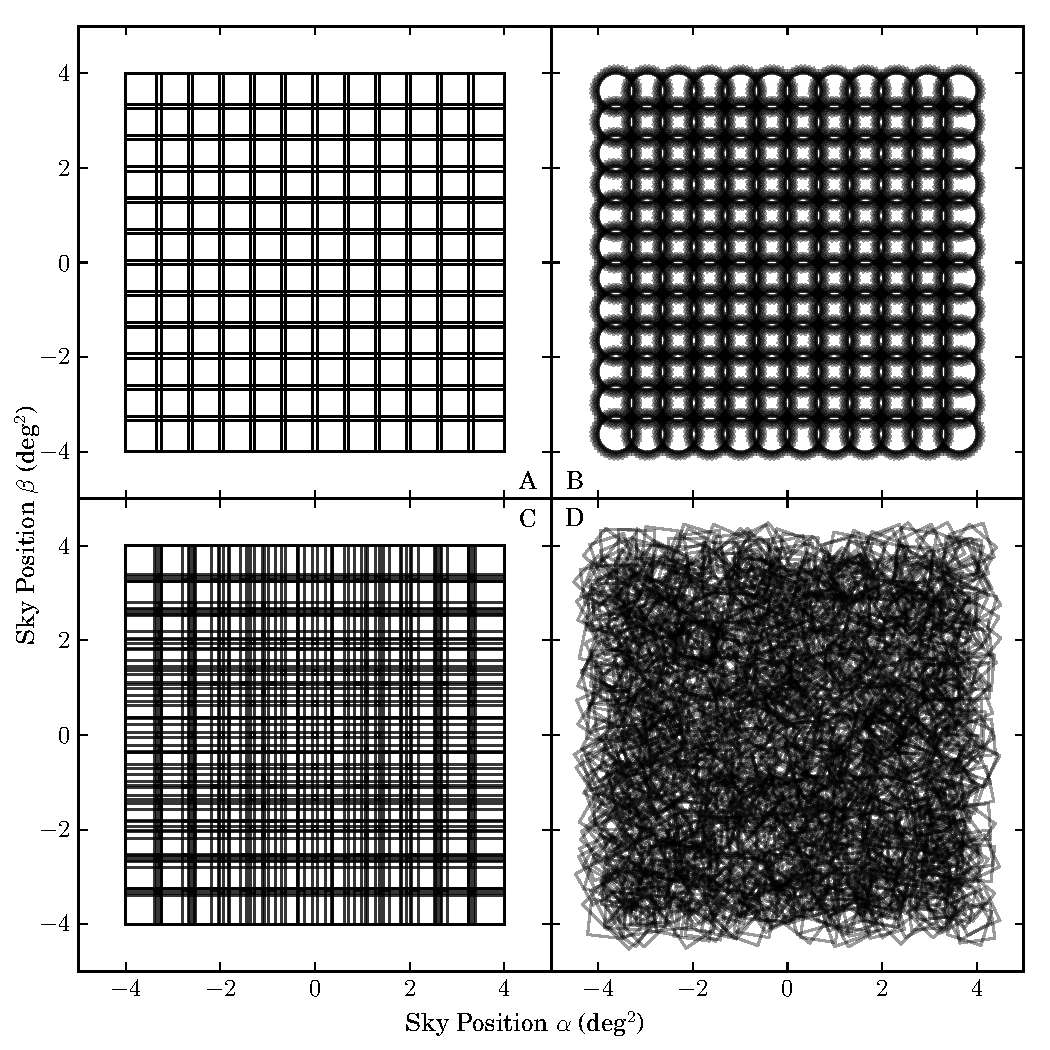
\includegraphics[height=\figureheight]{./1203.6255v2/simple_surveys.pdf}
\end{frame}
\begin{frame}
  \frametitle{imaging survey design {\footnotesize (Holmes, Hogg, Rix, arXiv:1203.6255)}}
  ~\hfill%
  \emph{A:}~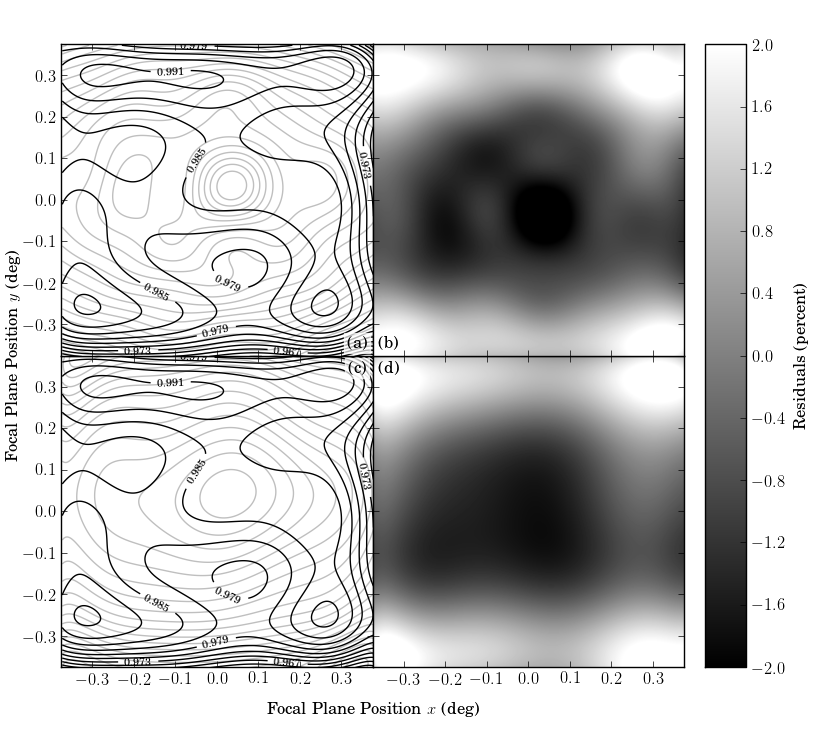
\includegraphics[height=\figureheight]{./1203.6255v2/A_5000_ff.png}
\end{frame}
\begin{frame}
  \frametitle{imaging survey design {\footnotesize (Holmes, Hogg, Rix, arXiv:1203.6255)}}
  ~\hfill%
  \emph{B:}~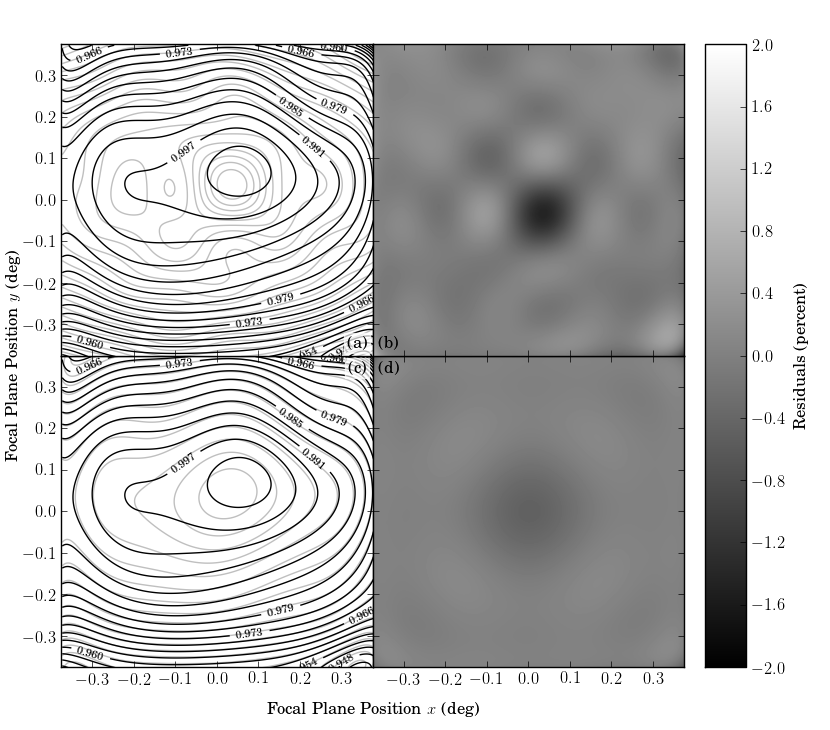
\includegraphics[height=\figureheight]{./1203.6255v2/B_1114_ff.png}
\end{frame}
\begin{frame}
  \frametitle{imaging survey design {\footnotesize (Holmes, Hogg, Rix, arXiv:1203.6255)}}
  ~\hfill%
  \emph{C:}~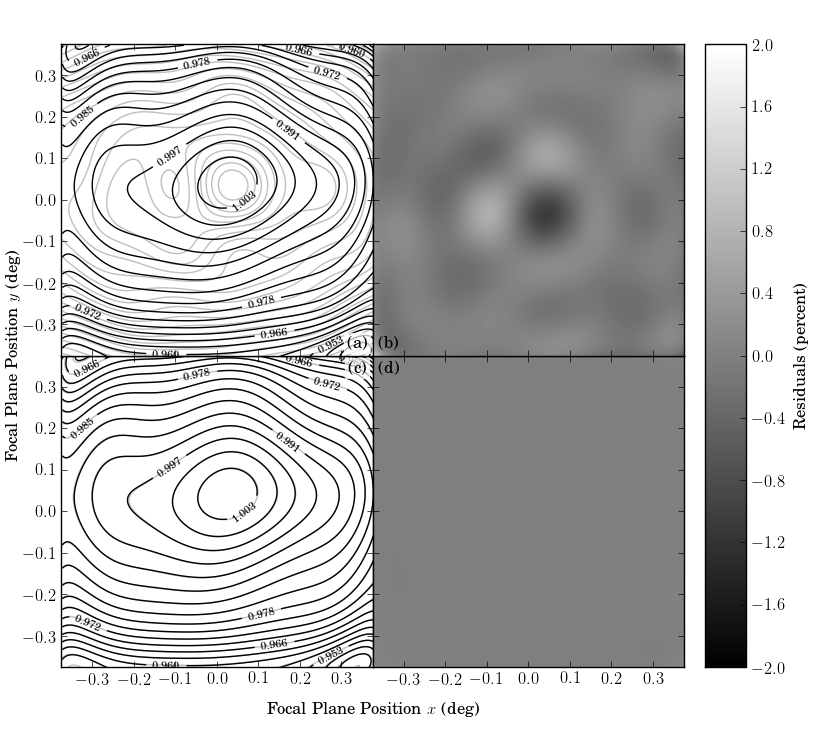
\includegraphics[height=\figureheight]{./1203.6255v2/C_24_ff.png}
\end{frame}
\begin{frame}
  \frametitle{imaging survey design {\footnotesize (Holmes, Hogg, Rix, arXiv:1203.6255)}}
  ~\hfill%
  \emph{D:}~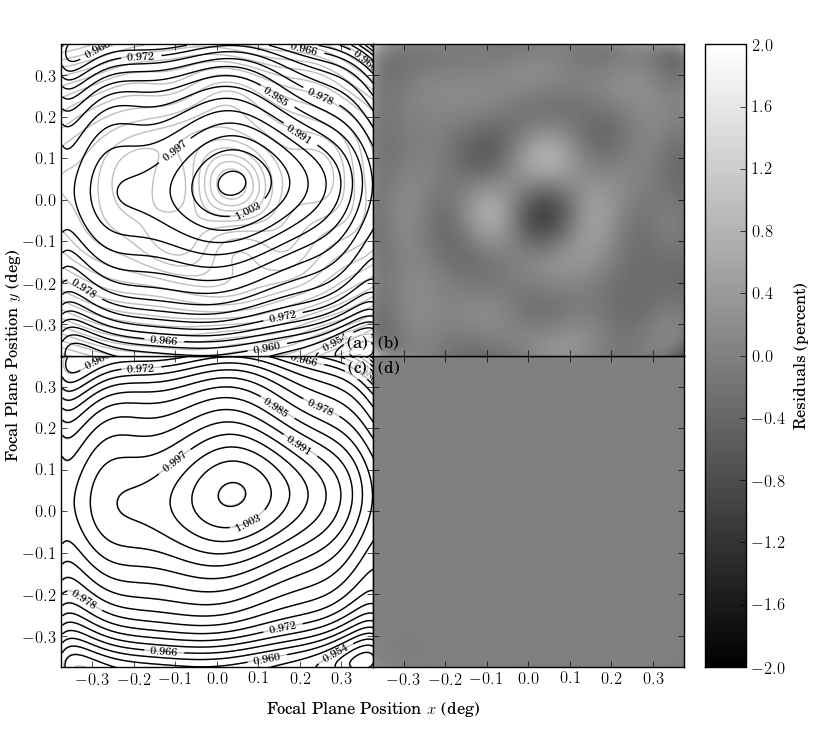
\includegraphics[height=\figureheight]{./1203.6255v2/D_11_ff.png}
\end{frame}
\begin{frame}
  \frametitle{imaging survey design {\footnotesize (Holmes, Hogg, Rix, arXiv:1203.6255)}}
  ~\hfill%
  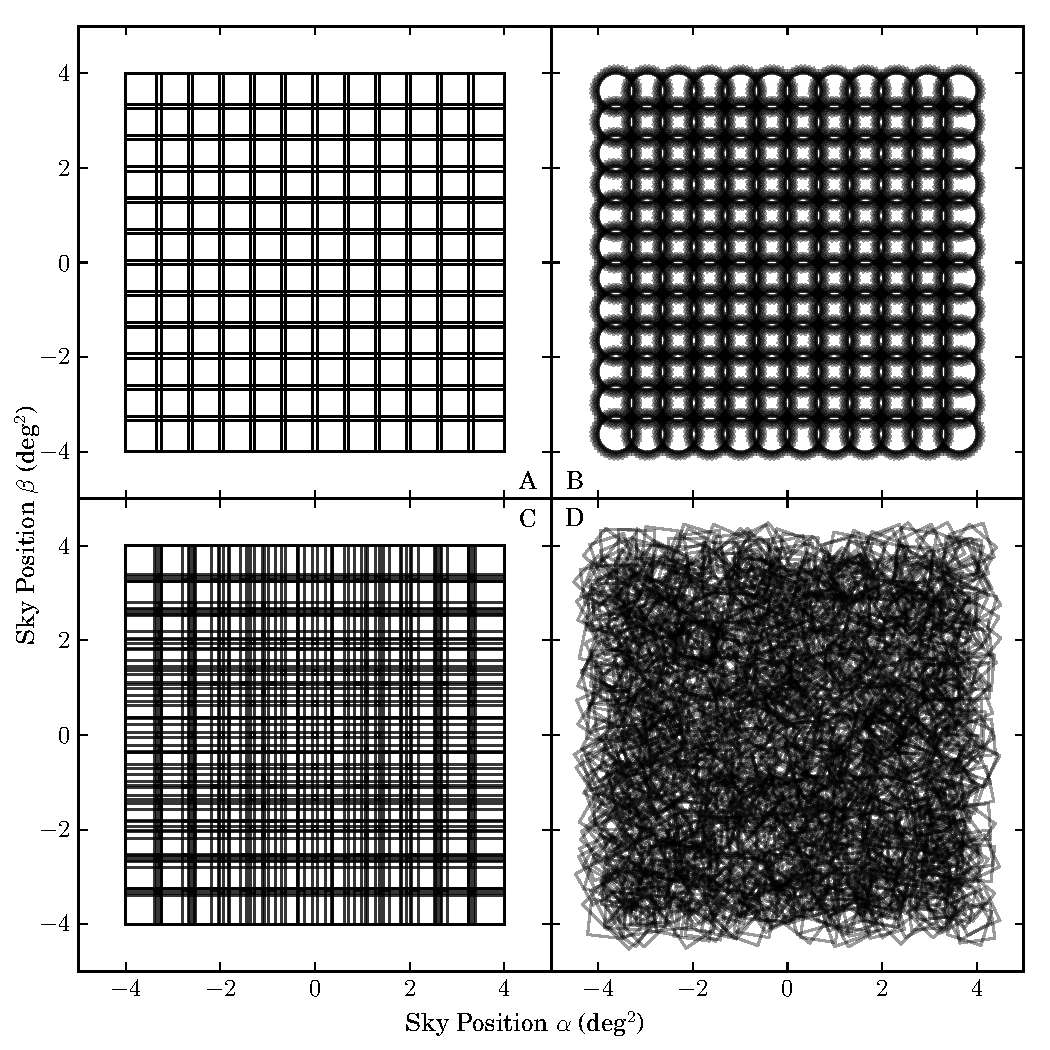
\includegraphics[height=\figureheight]{./1203.6255v2/simple_surveys.pdf}
\end{frame}

\begin{frame}
  \frametitle{imaging survey design: comments}
  \begin{itemize}
  \item recommend off-by-one and psuedo-random coverage patterns
    \begin{itemize}
    \item move the same star to different detector positions
    \item (give more uniform coverage than grids)
    \item (don't take additional time)
    \end{itemize}
  \item implementation challenges are \emph{social}
  \end{itemize}
\end{frame}

\begin{frame}
  \frametitle{radical self-calibration}
  \begin{itemize}
  \item What if you are never given any proper redundancy?
  \item What if you literally only look at any star in one detector location?
  \item What if there is no calibration program whatsoever?
  \end{itemize}
\end{frame}

\begin{frame}
  \frametitle{the NASA \kepler\ \& \kt\ Missions}
  \begin{itemize}
  \item deliberately try to fix stars in detector coordinates
    \begin{itemize}
    \item no redundancy (of the kind we want)
    \item pessimal for self-calibration
    \item no calibration program
    \end{itemize}
  \item most detector pixels never get telemetered down
    \begin{itemize}
    \item very sparse information on the focal plane
    \end{itemize}
  \item instrument and flat-field model not good enough
    \begin{itemize}
    \item routinely performing photometry with \emph{precision} around $10^5$
    \item \emph{!!}
    \end{itemize}
  \end{itemize}
\end{frame}

\begin{frame}
  \frametitle{radical self-calibration {\footnotesize (Wang \etal, in preparation)}}
  \begin{itemize}
  \item if a star's behavior can be predicted confidently by
    \emph{other stars} then that behavior must be being imprinted by
    the spacecraft
  \item using these ideas to separate spacecraft-induced from
    intrinsic stellar variability
  \end{itemize}
\end{frame}

\begin{frame}
  \frametitle{\kt\ calibration {\footnotesize (Foreman-Mackey \etal, arXiv:1502.04715)}}
  ~\hfill
  \includegraphics<1>[trim=100 100 100 100, clip, height=\figureheight]{brownbag/brownbagp10.pdf}
  \includegraphics<2>[trim=100 100 100 100, clip, height=\figureheight]{brownbag/brownbagp14.pdf}
  \includegraphics<3>[trim=100 100 100 100, clip, height=\figureheight]{brownbag/brownbagp15.pdf}
  \includegraphics<4>[height=0.9\figureheight]{1502.04715/figures-corr.pdf}
\end{frame}

\begin{frame}
  \frametitle{NASA \hst\ \wfc\ imaging {\footnotesize (Vakili, Fadely, Hogg, in prep)}}
  \begin{itemize}
  \item could we calibrate with no repeat observations of any kind?
  \item images have to be generated by mixtures of point sources!
  \item simultaneously model PSF and every scene
  \item residuals that are consistent in detector position are flat-field (or vignetting) issues.
    \begin{itemize}
    \item a calibration of \hst\ that makes no use whatsoever of any calibration observations
    \item relies on having many, many observations
    \item (currently vapor-ware)
    \end{itemize}
  \end{itemize}
\end{frame}

\begin{frame}
  \frametitle{related efforts}
  \begin{itemize}
  \item stellar parameter standards and spectroscopy
  \item CMB experiments
  \item spacecraft attitude determination
  \item exposure times and bandpasses and \foreign{etc.}
  \end{itemize}
\end{frame}

\conclusions

\end{document}
